% !TeX program = pdfLaTeX
\documentclass[12pt]{article}
\usepackage{amsmath}
\usepackage{graphicx,psfrag,epsf}
\usepackage{enumerate}
\usepackage{natbib}
\usepackage{textcomp}
\usepackage[hyphens]{url} % not crucial - just used below for the URL
\usepackage{hyperref}
\providecommand{\tightlist}{%
  \setlength{\itemsep}{0pt}\setlength{\parskip}{0pt}}

%\pdfminorversion=4
% NOTE: To produce blinded version, replace "0" with "1" below.
\newcommand{\blind}{0}

% DON'T change margins - should be 1 inch all around.
\addtolength{\oddsidemargin}{-.5in}%
\addtolength{\evensidemargin}{-.5in}%
\addtolength{\textwidth}{1in}%
\addtolength{\textheight}{1.3in}%
\addtolength{\topmargin}{-.8in}%

%% load any required packages here



% Pandoc citation processing

\usepackage{booktabs}
\usepackage{longtable}
\usepackage{array}
\usepackage{multirow}
\usepackage{wrapfig}
\usepackage{float}
\usepackage{colortbl}
\usepackage{pdflscape}
\usepackage{tabu}
\usepackage{threeparttable}
\usepackage{threeparttablex}
\usepackage[normalem]{ulem}
\usepackage{makecell}
\usepackage{xcolor}

\begin{document}


\def\spacingset#1{\renewcommand{\baselinestretch}%
{#1}\small\normalsize} \spacingset{1}


%%%%%%%%%%%%%%%%%%%%%%%%%%%%%%%%%%%%%%%%%%%%%%%%%%%%%%%%%%%%%%%%%%%%%%%%%%%%%%

\if0\blind
{
  \title{\bf Climate Change and Aging: A systematic Review}

  \author{
        Mathew E. Hauer \thanks{The authors gratefully acknowledge
\ldots{}} \\
    Department of Sociology, Florida State University\\
     and \\     Kyle Rose \\
    Department of Sociology, Florida State UniversityW\\
      }
  \maketitle
} \fi

\if1\blind
{
  \bigskip
  \bigskip
  \bigskip
  \begin{center}
    {\LARGE\bf Climate Change and Aging: A systematic Review}
  \end{center}
  \medskip
} \fi

\bigskip
\begin{abstract}
In this systematic review, we analyze the literature through Web of
Science's SCI-Expanded containing the words ``aging'' or ``aged'' and
``climate change'' and receiving at least four citations per year since
publication (n = 607 articles). After discarding irrelevant articles
(ie, ``aging infrastructure''), the 181 remaining articles
overwhelmingly (86\%) fall into two categories: temperature/mortality
(n=97; 69\%) and temperature/morbidity (n = 23; 17\%). However, many
other important climate topics related to aging remain underdeveloped.
Notably, adaptation (n = 8; 6\%), vulnerability (n = 5; 4\%),
emissions/mitigation (n = 4; 3\%), drought and mortality (n = 1; 0.7\%),
food security (n = 1; 0.7\%), and climate perceptions (n = 0) remain
understudied. Furthermore, more than half of the studies were conducted
in the United States (n = 30), China (n = 23), Globally (n = 16), and
Australia (n = 9), suggesting a paucity of information in the Global
South (n = 11) where climate impacts will be greatest. There were more
studies specifically on Spain (n = 5) than specifically on the entire
African continent (n = 4). Finally, 18 articles (13\%) offered
projections in some form, most to the middle of the century.
Gerontologists and aging scientists should look beyond the relationship
between heat and mortality to offer a more holistic view of aging and
climate change. {[}Sentence about Geography{]}. Prospective analyses, as
opposed to retrospective, could shed additional light on the link
between aging and climate change.
\end{abstract}

\noindent%
{\it Keywords:} 3 to 6 keywords, that do not appear in the title
\vfill

\newpage
\spacingset{1.45} % DON'T change the spacing!

\hypertarget{introduction}{%
\section{Introduction}\label{introduction}}

Two seemingly immutable trends will crash head-on during this century:
the global populace will continue to age and global climate change
impacts will worsen as the century progresses. By the end of the
century, when climate change impacts will be considerably more intense
than today, the Global populace exposed to these impacts will be
decidedly older, amplifying climate change impacts. Many of the
anticipated impacts from climate change disproportionately impact the
elderly versus younger, more vigorous age groups making these two trends
particularly potent when taken together.

Para: Focuses on Climate Change

Para: Focuses on Aging processes

Para: Gap bringing together (Climate Change and Aging)

Para: Research Questions with brief methods

\hypertarget{methods-and-materials}{%
\section{Methods and Materials}\label{methods-and-materials}}

We use a systematic literature review to assess the literature on
climate change and aging.

\hypertarget{document-selection}{%
\subsection{Document selection}\label{document-selection}}

We used a keyword search on Clarviate's Web of Science-expanded search
engine using the Boolean operator ``TS=(aging OR aged OR elderly) AND
TS=(``climate change'').'' We selected Web of Science due to its
comprehensive scientific coverage of peer-reviewed literature. We
conducted the search on September 7, 2022. This search retrieved an
initial universe of 16,828 articles. We filtered these results to
include articles of relatively high impact, defined subjectively as
those articles with at least four citations per year (n = 3,852). To
further isolate those articles pertaining to aging and climate change,
we further restricted our search to those articles containing the words
(aging or aged or elderly) in the abstract (n = 607).

We then reviewed these articles for relevance, discarding articles
concerning ``aging infrastructure'' or ``aging forests'' to isolate
articles on human aging and climate change. This yielded a total of 181
articles included in this systematic review
(\textbf{\autoref{fig-diagram}}).

\begin{figure}
\centering
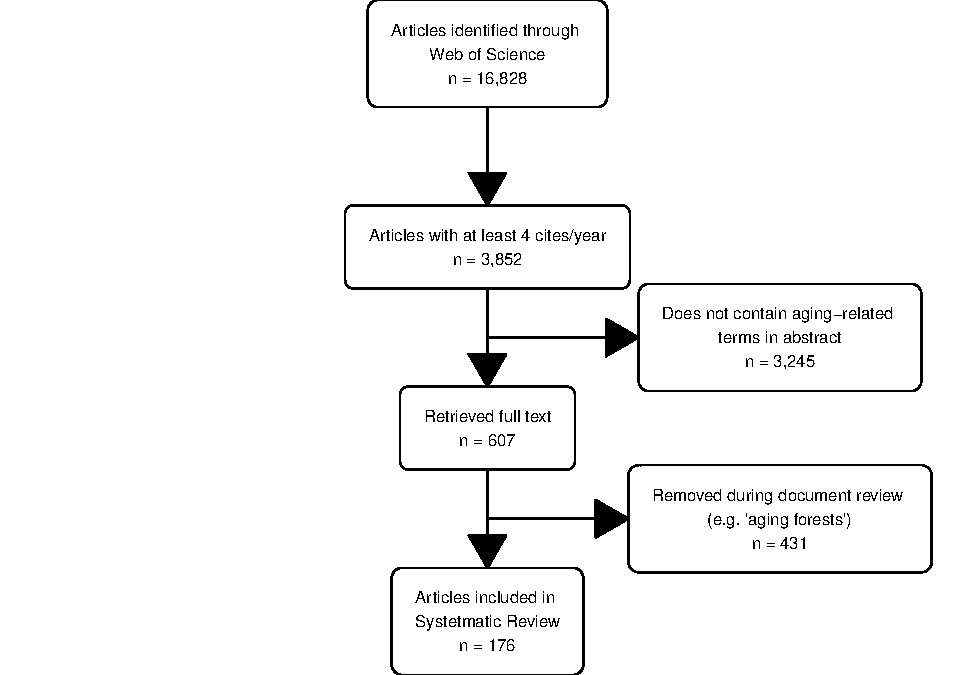
\includegraphics{MainDocument_files/figure-latex/figureflowdiagram-1.pdf}
\caption{PRISMA Flow Diagram. \label{fig-diagram}}
\end{figure}

\hypertarget{data-availability}{%
\section{Data Availability}\label{data-availability}}

The underlying computer code and data that support the findings of this
study are available in the Supplementary Material and have been
deposited in Zenodo (DOI).

\bibliographystyle{agsm}
\bibliography{bibliography.bib}

\end{document}
